\documentclass[tikz,border=10pt]{standalone}
\usepackage{tikz}
\usetikzlibrary{positioning, arrows}
\usetikzlibrary{decorations.pathreplacing}
\usetikzlibrary{calc}
\usepackage{pgfplots}
\usepgfplotslibrary{dateplot}
\tikzset{
  font=\small,
  node distance=0.5cm and 0.2cm,
  bdata/.style={draw, rectangle, text width=2.2cm, align=center},
  sdata/.style={draw, rectangle, text width=1.75cm, align=center},
  bmodel/.style={rectangle, fill=mLightBrown, text width=4cm, align=center, rounded corners},
  smodel/.style={rectangle, fill=mLightBrown, text width=2.2cm, align=center, rounded corners},
  pred/.style={draw, rectangle, text width=1cm, align=center}
}
\usepackage{xcolor}
\definecolor{mDarkTeal}{HTML}{23373b}
\definecolor{mLightBrown}{HTML}{EB811B}
\definecolor{mDarkBrown}{HTML}{B85002}
\definecolor{mLightGreen}{HTML}{14B03D}

\usepackage{fontspec}
\setmainfont{Mona Sans}

\begin{document}
  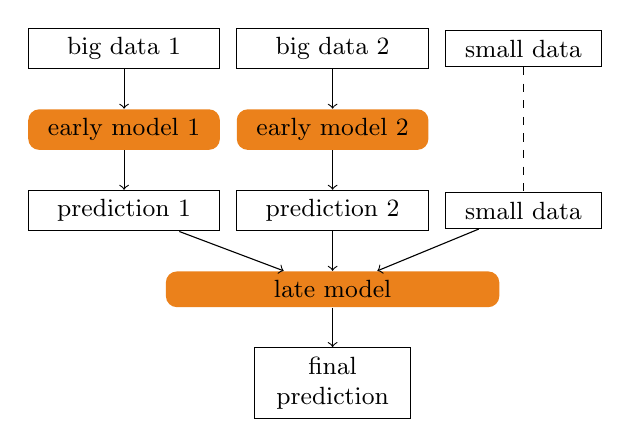
\begin{tikzpicture}  
    \node[bdata] (bigdata1) {big data 1};
    \node[bdata, right=of bigdata1] (bigdata2) {big data 2};
    \node[sdata, right=of bigdata2] (smalldata) {small data};
    \node[smodel, below=of bigdata1] (earlymodel1) {early model 1};
    \node[smodel, right=of earlymodel1] (earlymodel2) {early model 2};
    \node[bdata, below=of earlymodel1] (earlypred1) {prediction 1};
    \node[bdata, right=of earlypred1] (earlypred2) {prediction 2};
    \node[sdata, right=of earlypred2] (esmalldata) {small data};
    \node[bmodel, below=of earlypred2] (latemodel) {late model};
    \node[sdata, below=of latemodel] (latepred) {final prediction};
    
    \draw[->] (bigdata1) -- (earlymodel1);
    \draw[->] (earlymodel1) -- (earlypred1);
    \draw[->] (bigdata2) -- (earlymodel2);
    \draw[->] (earlymodel2) -- (earlypred2);
    \draw[dashed] (smalldata) -- (esmalldata);
    \draw[->] (earlypred1) -- (latemodel);
    \draw[->] (earlypred2) -- (latemodel);
    \draw[->] (esmalldata) -- (latemodel);
    \draw[->] (latemodel) -- (latepred);
  \end{tikzpicture}
\end{document}